We next consider a complex entire-muscle model involving motoneurons, sarcomeres and spindles.
The motoneurons and sarcomeres are used to model a \e{motorunit}, which is associated with a specific \e{fibre type} $\tau\in[0,1]$.
Here, $\tau=0$/$\tau=1$ corresponds to slow/fast twitch fibres, respectively.
We choose $\mups\in \N$ different motorunits in a ``motorunit-pool'', specified by $\tau_k,k=1\ldots\mups$.

\subsection{Motoneuron}
\cite{Cisi2008, negro2011}
The motoneuron model consists of $6$ degrees of freedom and reads as
\begin{align}
	\vq'(t) &= \fmo(\vq(t),\tau) + \ve_2\kappa(t)\nu(t,\tau) + \ve_2\nu_b(t) & \vq(0) &= \vnull,
\end{align}
for any fibre type $\tau$.
Here, $\ve_2\in\R^6$ is the second unit-vector, $\nu(t,\tau),\nu_b(t)$ describe noises (fibre-type dependent and base noise)
and $\kappa(t)$ an external input signal (e.g. from the central cortex).
This is used to activate/stimulate the motoneuron by addition to the second component $\fmo_2$, which describes the voltage change on the cell's soma.
The external signal $\kappa(t)$ can be seen as a \e{mean current}, as it imitates the overloaded signal from many firing distant neurons.
We will use $\vq^k(t) \in \R^6$ to indicate the current state of the $k$-th motoneuron (of the $k$-th motorunit).

\fix{motoneuron model parameter interpolation (coolExp)}
\fix{maximum mean input current!}

\subsection{Sarcomere}
The sarcomere model describes the force development inside a muscle fibre and is taken from \cite{Shorten2007}.
It has $56$ degrees of freedom and is given by
\begin{align}
	\vr'(t) &= \fsa(\vr(t),\tau) & \vr(0) &= \vr_0(\tau),
\end{align}
for any fibre type $\tau$.
There is a set of $105$ (fibre-type dependent) constants for the model, which we denote by $\csa(\tau)\in\R^{105}$.
We denote by $\vr^k(t)\in\R^{56}$ the state of the $k$-th sarcomere model (of the $k$-th motorunit).

\subsection{Spindle}
The spindle is the muscle component responsible for motoneuron feedback, where the model used is from \cite{Mileusnic2006}.
It has $9$ degrees of freedom and is given by
\begin{align}
	\vs'(t) &= \fsp(\vs(t),\dla(t),\eta(t)) & \vs(0) &= \vnull,\label{def:spindlesys}
\end{align}
where $\dla$ describes the change in fibre length and $\eta$ the frequency of an associated motoneuron.
We denote by $\vs^k(t)\in\R^9$ the state of the $k$-th spindle model. In real muscles, the number of spindles is independent from the
number of motorunits, but we use $\mups$ here for simplicity.

\subsection{Model connections}
The overall muscle model is
%
\begin{figure}[!htp]
    \begin{center}%
    \begin{tikzpicture}[auto,%
            block_assign/.style ={rectangle, draw=black, very thick, fill=white,%
            text width=10em, text centered, minimum height=3em, inner sep=6pt},%
            block_big/.style ={rectangle, draw=black, very thick, fill=white,%
            text width=14em, text centered, minimum height=3em, inner sep=6pt},%
            block_dashed/.style ={rectangle, draw=black, very thick, fill=white,%
            text width=10em, text centered, minimum height=3em, inner sep=6pt},%
        ]%
        \tikzstyle{stateEdgePortion} = [black, very thick, -latex', shorten >=1pt];
        \tikzstyle{stateEdge} = [stateEdgePortion];
        \tikzstyle{edgeLabel} = [pos=0.5, text centered];
        \tikzstyle{edgeLabelLow} = [pos=0.25, text centered];
        \tikzstyle{edgeLabelHigh} = [pos=0.25, text centered];
        \tikzstyle{line} = [draw, black, very thick, -latex', shorten >=1pt]];
        \tikzstyle{sline} = [draw, black, very thick];
        \tikzstyle{dline} = [draw, black, dashed, very thick, -latex', shorten >=1pt]];
        \tikzstyle{doublearrow} = [draw, black, very thick, <->, -latex', shorten >=1pt, shorten <=5pt, >=stealth]];
%        \tikzstyle{doubledline} = [draw, black, dashed, very thick, <->, -latex', shorten >=1pt, shorten <=5pt, >=stealth]];
        \node [block_big] (neuro)  {{\bf motoneurons} $\vq^k(t)$\\firing times};%
        \node [block_big, below of=neuro, node distance=30mm] (cell)  {{\bf half-sarcomeres $\vr^k(t)$}\\ action potential, active stress};%
        \node [block_dashed, left of=cell, node distance=80mm] (spindle)  {{\bf spindles $\vs^k(t)$} \\ electrical feedback};%
        \node [block_big, below of=cell, node distance=30mm] (mechanics)  {{\bf 3D continuum mechanics} \\ geometry, deformation};%
        \path [line] (neuro) -- (cell) node[edgeLabel]{$q^k_2(t)$};
        \draw (cell.south) edge[stateEdge] node[edgeLabel]{activation $\alpha(X,t) = \sum\limits_{k=1}^\mups w_k(X) r^k_{53}(t)$} (mechanics.north);
        \path [line] (mechanics) -| (spindle) node[edgeLabelHigh]{$\dla(X_k),\la''(X_k)$};
    	\path [line] ($(neuro.west) + (0,0.3)$) -| ($(spindle.north) + (-0.5,0)$);
    	\path [line] ($(spindle.north) + (0.5,0)$) |- ($(neuro.west) + (0,-0.3)$);
      	\node at (-5.7,-0.7) {$\gamma_{spin}(t)$};
    	\node at (-5.8,0.8) {$\eta(q^k_2(t))$};
    \end{tikzpicture}%
    \end{center}%
    \caption{Test}
\end{figure}

\subsubsection{Frequency detection}

\subsubsection{Motoneuron to Sarcomere}
The motoneuron soma signals $q^k_2(t)$ are used to provide activation spikes for the $k$-th sarcomere.
As the sarcomere model merely reacts to high spikes, the motoneuron output is scaled by a nonlinear function $\gamma$ to emphasize high peaks.
Essentially, the small signals are multiplied by a small factor $\beta_m = 0.3$, and the high signals are intensified by $\beta_M = 7$.
The transition from low to high factor is realized by a smooth Gaussian,
where we choose a threshold signal of $q_M = 40$ to pinpoint the signal from which on the $\beta_M$ factor is applied:
\begin{align}
	\gamma(q) &:= \begin{cases}
		\beta_m + e^{-(q-q_M)^2/150}(\beta_M-\beta_m), & 0 < q < q_M\\
		\beta_M & q \geq q_M,
	\end{cases}
\end{align}
Figure \ref{MSLink} illustrates the 
\begin{figure}[!ht]
	\centering
	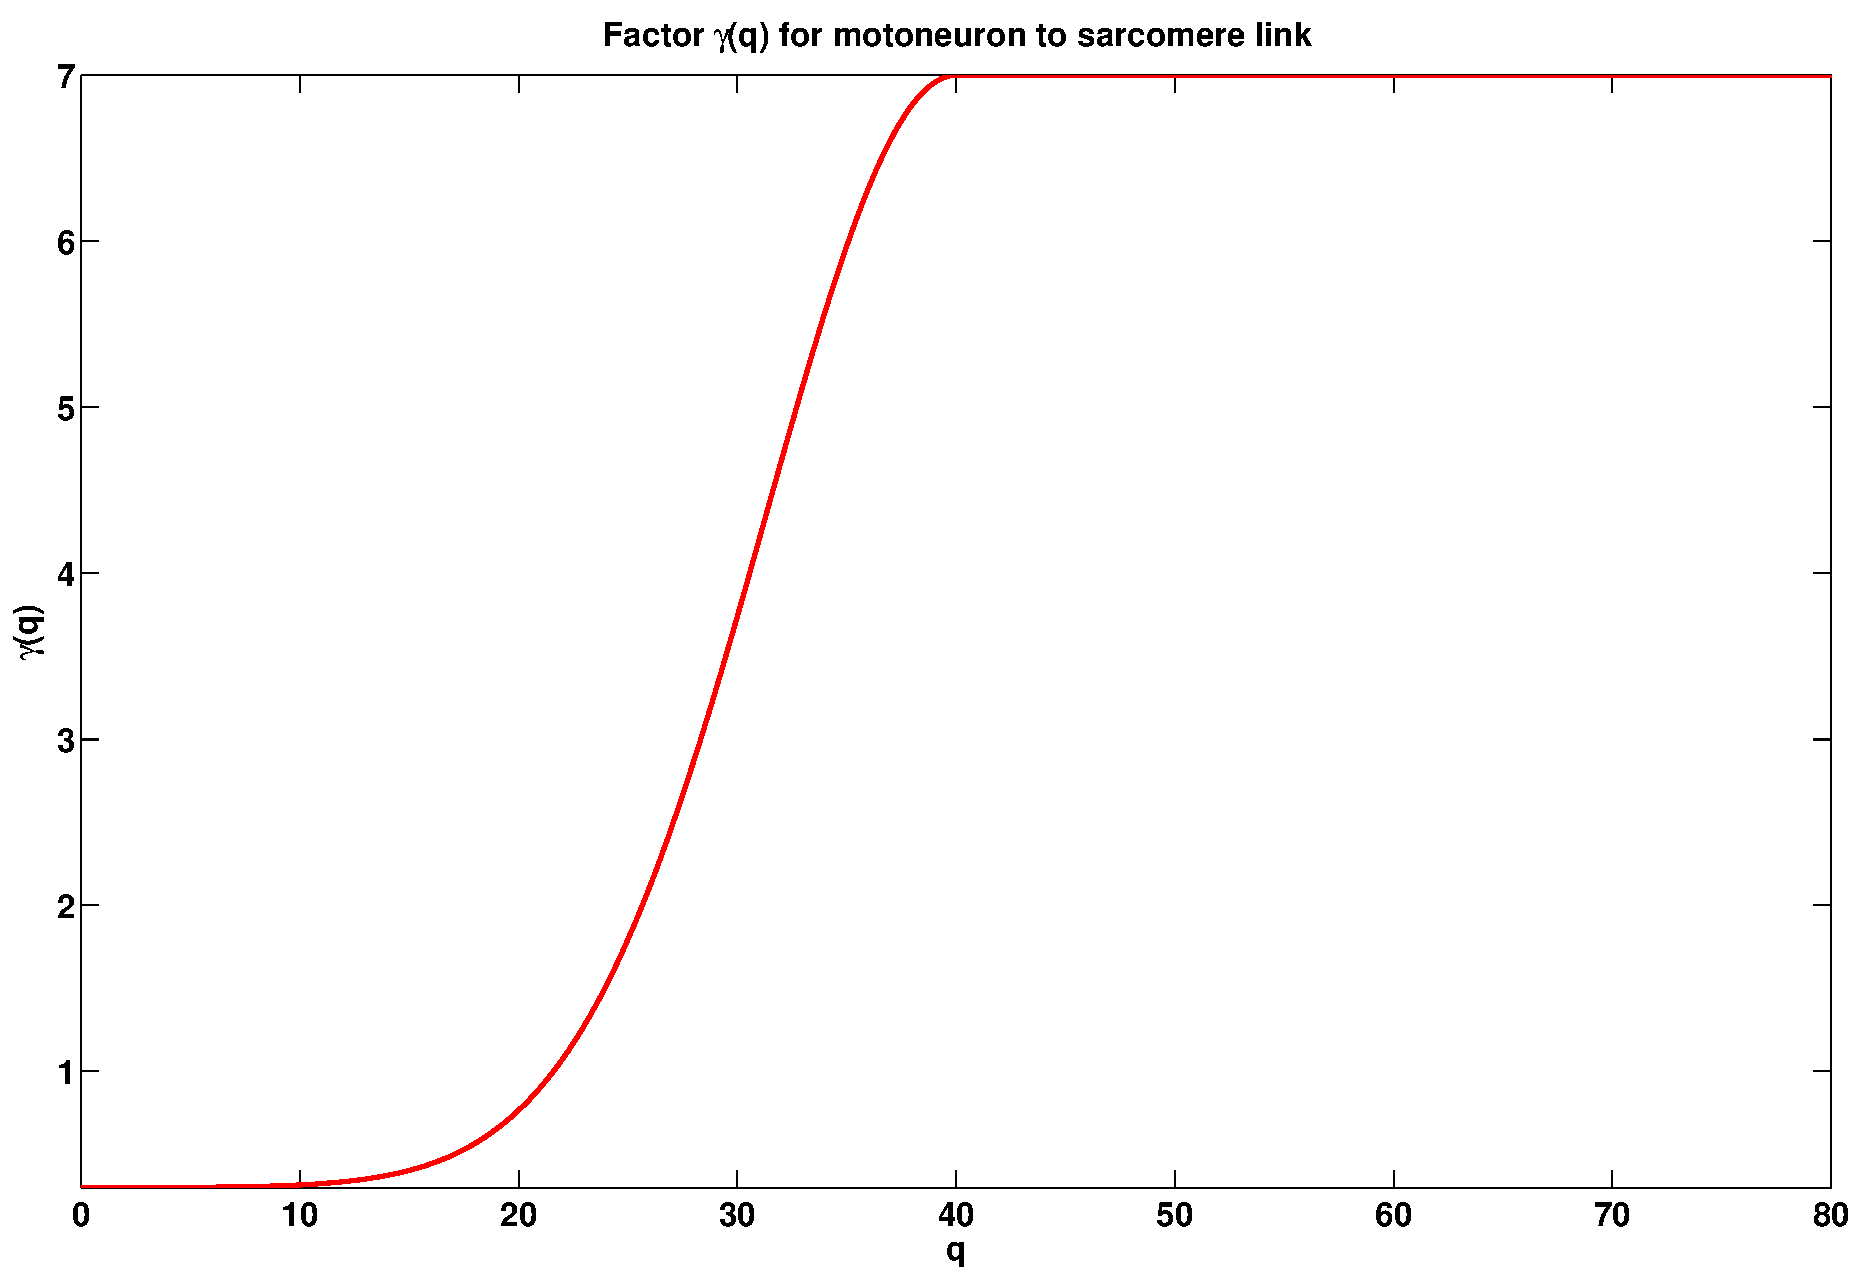
\includegraphics[width=\single]{moto_sarco_link_factor.pdf}
	\caption{Amplification factor for motoneuron signals}
	\label{fig:MSLink}
\end{figure}
Taking into account division by sarcomere model constants, the sarcomere models now read as
\begin{align}
	{\vr'}^k(t) &= \fsa(\vr^k(t),\tau_k) + \ve_1 \frac{\gamma(q_2^k(t))}{\csa_1(\tau_k)}q_2^k(t),
\end{align}
where $\ve_1 \in \R^{56}$ denotes the first unit vector, i.e. the signal is added to the first component of the sarcomere models.

\subsubsection{Sarcomere to Mechanics}
The sarcomere model component $\vr_{53}^k(t)$ is an indicator for the currently developed force in the muscle fibre.
\fix{hier das modell aus der diss erwähnen mit fasern und diffusion + erläuterung}
Within the mechanics FE-framework, this can be transformed to active stress $\alpha(X,t)$ in $\vSf$ by weighting of all $\mups$ force signals at spatial locations.
Hence, we make the ansatz
\begin{align}
	\alpha(X,t) = \sum\limits_{k=1}^\mups \frac{w_k(X)}{r^k_M} r^k_{53}(t).
\end{align}
Here, we introduce weight functions $w_k(X)$ for the fibre forces satisfying $\sum w_k(X) = 1 \fo X$.
Further, the constants $r^k_M\in\R$ are the maximum forces for each motorunit (i.e. $\tau_k$), determined by a long-time simulation of each sarcomere model using an
artificial $60Hz$ stimulation.
This ensures that $\alpha(X,t) \in [0,1] \fo X,t$. 

\subsubsection{Mechanics to Spindle}
According to \ref{def:spindlesys}, the spindle models use two external inputs:
The current change rate $\dla$ of fibre stretch and the motoneuron frequency $\kappa(t)$, where the latter will be discussed in Section
\ref{subsec:moto_spindle}.
As the fibre stretch is a local property of the continuum, we fix $\mups$ spindle locations $X_k\in\Omega$ and simply observe $\dla(X_k,t)$ to obtain the second
argument of the $k$-th spindle dynamics $\fsp$.
We recall the definition \ref{def:fibrestretch} and observe 
\begin{align*}
	\dla(X,t) &= \d{}{t}\no{\vF(X,t)\va_0(X)} = \frac{(\vF(X,t)\va_0(X))^T}{\no{\vF(X,t)\va_0(X)}}\d{}{t}\vF(X,t)\va_0(X)\\
	  &= \frac{1}{\la(X,t)}\va_0(X)^T\vF(X,t)^T\vF'(X,t)\va_0(X).
\end{align*}
Hence, if the $X_k$ are chosen among the set of all elements' Gauss integration points, quantities to compute $\dla$ are readily available during mechanics evaluation.

\subsubsection{Spindle to Motoneuron}
According to \cite{Mileusnic2006}, the spindle model has two algebraic scalar quantities called \e{primary} and \e{secondary afferents},
denoted by $\theta_p(\vs^k(t))$ and $\theta_s(\vs^k(t))$, respectively.
These afferents describe the firing frequency in [pps] of the spindle dendrites leading back into the motoneuron pool.
In a muscle, all spindles are connected to the entirety of the motoneuron pool \fix{ref?}, which will be modeled via averaging of all $\mups$ spindle's afferent outputs.
This gives a \e{mean spindle activation} of
\begin{align}
	\kappa^s(t) &:= \frac{1}{\mups}\sumjmups w_p\theta_p(\vs^j(t)) + w_s\theta_s(\vs^j(t))
\end{align}
which is added to the change rate of each motoneuron's soma alike the external mean current:
\begin{align}
	\vq'(t) &= \fmo(\vq(t),\tau) + \ve_2(\kappa(t) + \kappa^s(t))\nu(t,\tau) + \ve_2\nu_b(t).
\end{align}    
% [6{:}8] , where the \ML-like notation indicates which components of the spindle states $\vs$ are used as arguments.

\subsubsection{Motoneuron to Spindle}\label{subsec:moto_spindle}
